\documentclass{article}
% Change "article" to "report" to get rid of page number on title page
\usepackage{amsmath,amsfonts,amsthm,amssymb}
\usepackage{setspace}
\usepackage{Tabbing}
\usepackage{fancyhdr}
\usepackage{lastpage}
\usepackage{extramarks}
\usepackage{url}
\usepackage{chngpage}
\usepackage{longtable}
\usepackage{soul,color}
\usepackage{graphicx,float,wrapfig}
\usepackage{enumitem}
\usepackage{morefloats}
\usepackage{multirow}
\usepackage{multicol}
\usepackage{indentfirst}
\usepackage{lscape}
\usepackage{pdflscape}
\usepackage{float}
\restylefloat{table}
\usepackage{algorithm}
\usepackage{algorithmic}
%\usepackage{natbib}
\usepackage[toc,page]{appendix}
%\providecommand{\e}[1]{\ensuremath{\times 10^{#1} \times}}

% In case you need to adjust margins:
\topmargin=-0.45in      % used for overleaf
%\topmargin=0.25in      % used for mac
\evensidemargin=0in     %
\oddsidemargin=0in      %
\textwidth=6.5in        %
%\textheight=9.75in       % used for mac
\textheight=9.25in       % used for overleaf
\headsep=0.25in         %

% Homework Specific Information
\newcommand{\hmwkTitle}{Progress Report 1}
\newcommand{\hmwkDueDate}{Monday,\ September\  24,\ 2018}
\newcommand{\hmwkClass}{Final Project}
\newcommand{\hmwkClassTime}{CSE 597}
\newcommand{\hmwkAuthorName}{Sahithi\ Rampalli}
\newcommand{\hmwkNames}{svr46}

% Setup the header and footer
\pagestyle{fancy}
\lhead{\hmwkNames}
\rhead{\hmwkClassTime: \hmwkTitle} 
\cfoot{Page\ \thepage\ of\ \pageref{LastPage}}
\renewcommand\headrulewidth{0.4pt}
\renewcommand\footrulewidth{0.4pt}

%%%%%%%%%%%%%%%%%%%%%%%%%%%%%%%%%%%%%%%%%%%%%%%%%%%%%%%%%%%%%
% Make title

\title{\vspace{2in}\textmd{\textbf{\hmwkClass:\ \hmwkTitle}} \\
\vspace{0.1in}\large{ \hmwkClassTime}\vspace{3in}}

\author{\textbf{\hmwkAuthorName} \\ \vspace{0.1in}
\hmwkDueDate }
\date{} % to take away today's date

%%%%%%%%%%%%%%%%%%%%%%%%%%%%%%%%%%%%%%%%%%%%%%%%%%%%%%%%%%%%%

\begin{document}
\begin{spacing}{1.1}
\maketitle

\newpage
\section*{Abstract}

The purpose of this project is to learn and build an optimized iterative solver for the discrete Poisson Equation on caretesian grid.
I chose to use Cholesky decomposition ($LDL^T$ fatorization) as direct method and Conjugate Gradient as iterative method to solve {Ax=b}.
The results of this project will be used for our research work where we implemented conjugate gradient solver for the same problem on FPGA architecture \cite{FPGACG}. We are trying to investigate various optimization techniques to come up with an efficient implementation of the solver which can be used in many scientific applications. It is more a mathematical problem than physical problem and we do not target a specific application. The aim is to compare the performance of the solver on different architectures including CPU and FPGA.
\section{Problem of Interest}

Finite difference numerical method is used to discretize the 2-dimensional poisson equation. On an m{x}n grid, it takes the form
\[(\nabla^2	u)_{ij} = \dfrac{1}{dx^2}(u_{i+1,j} + u_{i-1,j} + u_{i,j+1} + u_{i,j-1} - 4u_{i,j} ) \] 
Discrete Poisson equation arises in various fields of study such as heat flow, electrostatics, gravity, computational fluid dynamics, theory of markov chains and many more. They occur frequently in scientific computing, for instance, when solving partial diferential equations, in inexact newton methods for solving optimization problems in machine learning applications etc. The size of the grids on which the equation is applied can go as large as 10s or 100s of 1000s. For such large matrix sizes, it is clearly essential to parallelize and optimize the solvers. Hence, an efficient implementation of CG which can be used in various physical applications is necessary. For our research, we have not chosen a specific physical problem, but would like to contribute possible optimization techniques for this iterative solver. However, for the convergence test, we use a tolerance to control the number of iterations. The convergence criteria is discussed in the next section.\\
\\
	For direct solver methods, banded LU (a special case of Gaussian Elimination) is the optimal method as the matrix in this problem is a diagonal matrix. Further optimization can be done by using $LDL^T$ factorization.
	Since the matrix sizes are really large, direct solvers are usually not preferred as $A^{-1}$ computation or back filling will be quite expensive. Iterative methods like  Jacobi, SOR, Conjugate Gradients are used to solve discrete Poisson Equation \cite{Berkley1996} . Iterative methods use the idea of nearest-neighbour computing to solve the equation. Methods like FFT and Multigrid can be faster than the iterative methods as they forward the information to points on the grid which are farther than the nearest neighbours. FFTs and multigrid are more specialized to solve problems like poisson, unlike direct solvers like LU decomposition which is used to solve almost any linear system (nonsingular). \cite{FFTPoisson}
\\
	We have a simple MATLAB implementation of Conjugate Gradient. We used it to compare the accuracy of our FPGA implementation. I have also used it to compare the accuracy of direct solver and serial CG implementations. Pseudo codes of $LDL^T$ decomposition and CG are shown in algorithms \ref{algoLDL} and \ref{algoCG}. I am using the MATLAB implementation to compare the convergence of every implementation of CG (parallel, GPU execution).
\subsection{Numerical Set-up}

\subsubsection{Direct Solver}
	I obtained the $A$ matrix for $LDL^T$ factorization using the MATLAB command "gallery('poisson', $n$)" where $n$ is the compute grid dimension which is half of the matrix dimension (say $N$). This MATLAB command generates the matrix based on the poisson equation discussed in section 1. The vector $b$ is populated with random numbers. As I am not focussing on a particular physical problem, using a random $b$ vector is meaningful. This would not affect the analysis or possible optimizations that we are investigating in any way. The same vector is used for both the solvers.

\subsubsection{Iterative Solver}
	For iterative solver, the matrix $A$ is not stored, but every matrix operation is visualized as a stencil operation computed on a grid of dimension $n$ which is half of the matrix dimension ($N$). The stencil operation is discussed in detail in the next section. The vector $b$ is same as that for direct solver.
\\
\newline
 The direct solver involves matrix vector multiplications. Without any optimizations, it is quite compute intesive to scale the problem to larger dimensions. Hence, for testing purposes, I chose matrix of sizes $64x64$, $256x256$ and $1024x1024$. The matrix dimensions for production problem can go upto 10s and 100s of 1000s. For our research work on FPGA, we used maximum matrix size of $10816x10816$. I claim that with multi-threading and matrix decomposition, the matrix dimension can go upto the order of $10^4$.
 \\
 For the applications of discrete poisson equation, the matrix dimensions can be of the order of $10^4$ or $10^5$. Due to the resource constraints (for storing larger matrices), I only use matrix dimensions upto order of $10^3$ to analyze the performance and then estimate the performance of serial solvers for larger dimension matrices.
\\
As mentioned, we are not targetting any particular physical problem. We mainly focus on the possible optimizations for the most compute intensive parts of the algorithms. Hence, we do not use any boundary conditions as they can be taken care during pre-processing or post-processing steps of the direct/iterative solver. For example, to solve the poisson's equation in an electrostatic setup, 
$\rho = \nabla^2\phi$,
for dirichlet boundaries $\phi(0) = D$, the condition can be implemented in the initial guess of the solution \cite{stackexchangeBoundary}. Hence, handling the boundary conditions is primarily dependent on the application.
\section{Solvers}

\subsection{Direct Solver}

As mentioned in the previous section, I use $LDL^T$ factorization as a direct solver for solving discrete poisson equation on large compute grids. An example of the poisson problem is shown in the figure \ref{poisson}.

\begin{center}
	\begin{figure}[H]
	\centering
       \includegraphics[scale=.40]{poisson.png}
        \caption{\label{poisson} Discrete Poisson Problem on 4x4 grid \cite{Berkley1996}.} 
	\end{figure}
\end{center}

Clearly the matrix can be viewed as a symmetric, banded matrix. When a matrix is symmetric, Cholesky decomposition ($LL^T$ factorization) is the optimal way to solve the linear system of equations. Since the above matrix is not only symmetric, but also diagonal dominated, a different version of Cholesky, $LDL^T$ factorization, is the best choice. 
If a matrix $A\epsilon R^{nxn}$ is symmetric and the principal submatrix $A(1:k,1:k)$ is nonsingular for $k=1:n-1$, then there exists a unit lower matrix $L$ and a diagonal matrix $D$ such that $LDL^T$ and the factorization is unique. \cite{MatComp}

The algorithm for $LDL^T$ factorization is shown in listing \eqref{algoLDL}. Here the matrix $A$ is overwritten with $D_i$ for $i=j$ and $L_{ij}$ for $i>j$.
\begin{algorithm}[H]

%\begin{multicols}{2}
\begin{algorithmic}[1]
%\caption{function [A, x, b] = LDLt(A, b)}

%\label{alg:seq}
\FOR{$j=1:n$}
\FOR{$i=1:j-1$ until convergence}
\STATE $v(i) = A(j,i)*A(i,i)$ 
\ENDFOR
\STATE $A(j,j) = A(j,j) - A(j,1:j-1).v(1:j-1)$
\STATE $A(j+1:n,j) = (A(j+1:n, j) - A(j+1:n,1:j-1).v(1:j-1))/A(j,j) $ 
%\STATE $resVec = [resVec, norm(A * x - b)]$ 
%\STATE $j \gets j + 1$	
\ENDFOR
%\STATE $its = j$
\end{algorithmic}
%\end{multicols}
\caption{\label{algoLDL} function [A, x, b] = $LDL^T(A, b)$} 
\end{algorithm}

The algorithm $LDL^T$ factorization requires about $n^3/3$ flops which is almost half the number of flops required for Gaussian Elimination. 

The implementation is also made memory-efficient by writing back to the matrix $A$ and vector $b$ and not using any other extra space. I also made an attempt to store $A$ as a banded matrix to reduce the space further. However, the logic did not work perfectly. I shall work on the logic and update the code in the coming days.

\subsubsection*{Timing and Memory}
For test problem, the chosen sizes of matrix A are $64x64$, $256x256$, $1024x1024$. The production problem size can be as large as $10861x10861$. 
The execution times for different test sizes upon using the G++ compiler optimization flag -O2 is shown in Table \ref{exec_direct}. The flag O2 has been chosen as it mainly optimizes for execution time and memory usage which are the important performance metrics I chose. I obtain similar performance with O3 flag and deproved performance with O1 flag. 
The memory required for matrix $A$ and vector $b$ is estimated in Kilobytes (KB). I obtained the virtual resident memory used by the task by executing the top unix command. 

\begin{table}[H]
\begin{center}
%\resizebox{\columnwidth}{!}{%
 \begin{tabular}{| c | c | c | c |} 
 \hline
$N$ & $Exec time (microseconds)$  & $Estimated Memory (KB)$ & $Memory (MB)$  \\ %[0.3ex] 
 \hline
64 & 758 & 16.25 & 2.42  \\ %\hline
256 &  18680 &257 & 3.11 \\ %\hline 
1024 &  1151817 & 4100 & 5.24 \\ %[0.3ex]
 \hline
\end{tabular}%
%}
\end{center}
\caption{\label{exec_direct} The execution time and number of elements stored for different test problem sizes.  } 
\end{table}

The execution time for back filling is shown in Table \ref{backfill_direct}.

\begin{table}[H]
\begin{center}
%\resizebox{\columnwidth}{!}{%
 \begin{tabular}{| c | c |} 
 \hline
$N$ & $Exec time (microseconds)$ \\ %[0.3ex] 
 \hline
64 & 74  \\ %\hline
256 &  372 \\ %\hline 
1024 &  10503  \\ %[0.3ex]
 \hline
\end{tabular}%
%}
\end{center}
\caption{\label{backfill_direct} The execution time for back filling for different test sizes.  } 
\end{table}

We can see that apart from the time for decomposition, the backfilling also takes considerable number of FLOPs and hence the execution time. 

The projection of execution time for production problem size $10816$x$10816$ is expected to be of the order of $10^8$ microseconds. The projection of memory for production problem size $10816$x$10816$ is estimated to be around 446.3 MB. Thus the space required grows exponentially with the problem size.


\subsection{Iterative Solver}

I use Conjugate Gradient (CG) method as an iterative solver for solving discrete poisson equation. One reason for choosing conjugate gradient is that it was developed for symmetric and positive definite matrices which is the case in the chosen problem. Also, as we are testing conjugate gradient on FPGA architecture, it would be useful to use this method and test it on CPU to compare the performance of our hardware design for CG with that on CPU.

Convergence criteria: I have chosen the tolerance to be of the order of $10^{-4}$. Most applications allow a tolerance upto order of $10^{-4}$ to $10^{-6}$. Even though I am not addressing a specific application, the choice of tolerance will not affect the trend in the performances of different matrix sizes as it will only increase the number of iterations. My inequality to test for convergence is:
\[ delta = dotProduct(residual_values); \epsilon = 0.0001 \]
\[ log_{10}(\sqrt{|delta|}) >= log_{10}(\epsilon) \]


\begin{algorithm}[H]

%\begin{multicols}{2}
\begin{algorithmic}[1]
%\caption{function [A, x, b] = CG(A, b)}

%\label{alg:seq}
\STATE $n = \text{size}(A,1)$ 
\STATE $x = \text{zeros}(n,1)$
%\STATE $resVec = [\hspace{1mm}]$
\STATE $r_{\text{old}} = b$ ; $p = r_{\text{old}}$ ; $j = 1$
\FOR{$i=1$ until convergence}
\STATE $z = A*p$ 
\STATE ${\alpha} = (r_{\text{old}}, r_{\text{old}})/(z, p)$
\STATE $x = x + \alpha * p$ 
\STATE $r = r_{old} - \alpha * z$
\STATE $\beta = (r, r) \, / \, (r_{\text{old}}, r_{\text{old}})$
\STATE $p = r + \beta* p$;
\STATE $r_{\text{old}} = r$
%\STATE $resVec = [resVec, norm(A * x - b)]$ 
%\STATE $j \gets j + 1$	
\ENDFOR
%\STATE $its = j$
\end{algorithmic}
%\end{multicols}
\caption{\label{algoCG} function [A, x, b] = stdCG(A, b)} 
\end{algorithm}

The Conjugate Gradient algorithm shown in \eqref{algoCG} has a matrix-vector multiplication operation $z=A*p$. However, one can view this operation as a stencil operation applied on the vector $p$. The stencil will be:
\begin{tabular}{|c|c|c|}
\hline
0 & -1 & 0\\ \hline
-1 & 4 & -1 \\ \hline
0 & -1 & 0 \\ \hline
\end{tabular}

This can be very easily deduced from the discrete poisson form shown in section 1.
Applying the stencil operation reduces the number of FLOPs exponentially as the stencil is computed on vector $p$ which is square root times the size of matrix $A$.
Performing $z=A*p$ as a stencil operation is not only compute-efficient but also memory-efficient as we do not have to store matrix $A$.

The convergence plot of $Log_{10}(Residual Values)$ Vs. $iterations$ is shown in the figure \ref{convPlot}. The plot is the same for all types of input initializations. I have tested the convergence of the solver for different and random input initializations including zero initialization and initialization based on a guess. Any type of initialization results in the same residuals values and hence the same convergence plot. (This has been tested multiple times.)
\begin{center}
	\begin{figure}[H]
	\centering
       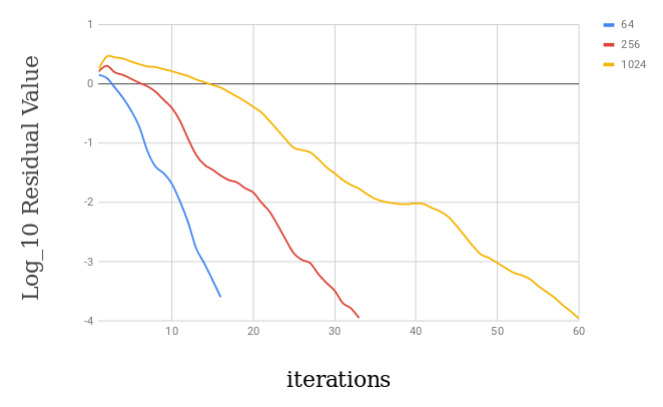
\includegraphics[scale=.40]{convergence.png}
        \caption{\label{convPlot} Convergence Plot} 
	\end{figure}
\end{center}


\subsubsection*{Timing and Memory}
For test problem, the chosen sizes of matrix $A$ are $64x64$, $256x256$, $1024x1024$. The production problem size can be as large as $10861x10861$. 
The execution times for different test sizes upon using the G++ compiler optimization flag -O2 is shown in Table \ref{exec_iter}. The flag O2 has been chosen as it mainly optimizes for execution time and memory usage which are the important performance metrics I chose. I obtain similar performance with O3 flag and deproved performance with O1 flag. Table \ref{exec_iter} also shows the estimated memory (in KB) and the memory required by the task (in MB). The memory estimation is based on the number of elements stored. 

I have tested the problem for different initializations for vector $x$. Any random initialization (tested multiple times) gives the same set of residual values and number of iterations. The possible reason is that the residual vector $r$ in conjugate gradient method is not much dependent on the values of $x$, which is evident from algorithm \eqref{algoCG}.

\begin{table}[H]
\begin{center}
%\resizebox{\columnwidth}{!}{%
 \begin{tabular}{| c | c|c|c|c|} 
 \hline
$N$ & $ExecTime (microseconds)$  & $Estimated Memory (KB)$ & $Memory (MB)$ \\ %[0.3ex] 
 \hline
64 & 155 &  1.25 & 0.97\\ %\hline
256 &  440 & 5 & 1.15\\ %\hline 
1024 &  4988 & 20 & 1.2\\ %[0.3ex]
 \hline
\end{tabular}%
%}
\end{center}
\caption{\label{exec_iter} The execution time and memory in KB for different test problem sizes.  } 
\end{table}

The size of the vector $b$ required for the problem increases linearly with the problem size.
The projection of execution time for production problem size $10816$x$10816$ is expected to be of the order of $10^6$ microseconds. The projection of memory for production problem size $10816$x$10816$ is expected to be around 212KB. Thus the space required grows linearly with the problem size. 

\section{Solver Comparison}

The table \ref{speedup} shows the speedup of the Conjugate Gradient method over the direct solver. Clearly, conjugate gradient method outperforms direct solver as the number of computations has reduced exponentially. Also, the speedup increases with increase in the matrix size.

From storage point of view, iterative solver wins over direct solver as the matrix $A$ is not stored in the former case (sparse matrix-vector multiplication operation is replaced by stencil operation). The number of elements required for CG increases linearly with problem size unlike the direct method where the growth is exponential.

Even for a production scale problem where matrix size is of the order $10^4$ and more, conjugate gradient will have greater speedup when compared to $LDL^T$ factorization.

It is clear that the execution time of direct solver, for production size problem is of the order of minutes which is pretty slow. Upon parallelizing the $LDL^T$ factorization, the matrix can be distributed among multiple threads for computation and the performance can be improved. Since, there may not be much communication/boundary sharing, the speedup due to parallelization can be close to the number of threads.

Also, for direct solver, the static memory allocation limits the size of the problem to be of the order $10^3$. As projeced in section 2.1, the memory requirement for production problem size is around 500MB which is too high for such applications. Nevertheless, the need for large space is eliminated in the iterative solver. For larger problems of order $10^5$ and higher, the memory required can be greater than 50MB and the processing time can be close to one minute. This can be improved by parallelizing the problem.

\begin{table}[H]
\begin{center}
%\resizebox{\columnwidth}{!}{%
 \begin{tabular}{| c | c |} 
 \hline
$N$ & $Exec time (microseconds)$  \\ %[0.3ex] 
 \hline
64 & 4.8x \\ %\hline
256 & 42.5x \\ %\hline 
1024 &  231x \\ %[0.3ex]
 \hline
\end{tabular}%
%}
\end{center}
\caption{\label{speedup} The speedup of CG over $LDL^T factorization$  } 
\end{table}

\section{Discussion and Conclusions}
In this report, I tried to solve the discrete Poisson Equation on caretesian grid. I showcase two methods to solve this problem - Direct method using $LDL^T$ factorization and Iterative method using Conjugate Gradient method. As mentioned earlier, I want to use this analysis and results to compare the performance of Conjugate Gradient method for solving discrete Poisson Equation on FPGAs. We chose to solve a more general mathematical problem, without focussing on any particular applications as we would only like to investigate the possible optimizations in the major bottleneck operations of the solver. By performing the required pre-processing and post-processing steps, these solutions can be slightly modified to solve any physical problem. Here, I only try to solve the mathematical problem. \\

For direct solver methods, banded LU (a special case of Gaussian Elimination) is the optimal method as the matrix in this problem is a diagonal matrix. Further optimization can be done by using $LDL^T$ factorization, a variant of LU factorization. For iterative method, I used Conjugate Gradient method as it is simpler. Also, we are using CG for our FPGA implementation. Hence, I can use these results and analysis for comparison of CPU and FPGA implementation.\\

From the results it can be concluded that iterative solvers are much better in terms of execution time and memory required than the direct solvers for solving discrete Poisson Equation. However, for production size problems which are of the order of $10^4$ to $10^6$, the processing time would be close to a minute and the space required will be around 50MB which cannot be afforded for the applications of discrete Poisson problem. Thus, it is required to parallelize this problem to improve on the processing time and allocate more resources to accomodate for the problem size\\

From parallelization perspective, Conjugate Gradient is easier to implement in this case as it mostly involves point-wise operations like dot product, vector addition and one stencil operation. The Direct method involves Matrix vector product. Hence, the matrix has to be carefully decomposed. From performance and space complexity point of view, Conjugate gradient will again outperform due to the exponentially smaller vectors stored in contrast to the matrix in direct method.

\newpage
\begin{appendices}

\section{Acknowledgements}

I would like to acknowledge my advisor at IIIT-Hyderabad, India for guiding me to work on conjugate gradient solver for poisson equation on different architectures. I would like to acknowledge my class mates, Chirag Satish and Amatur Rahman, for helping me fix some implementation errors and clarifying some doubts regarding compute nodes on ACI.

\section{Code}

The code is available of GitHub and can be obtained by cloning:
git clone https://github.com/sahithi-rv/ProjectReport1.git
I would continue to host the code on GitHub as it is a free software. Also, I would like to periodically update the repository with any further optimizations I could make to the problem or use any of the upcoming linear algebra libraries. Hosting it on GitHub would make the task easier as the updates can be carefully tracked. Also, this work would be helpful for anyone interested in this field of research and one can fork the repository and modify the code as they require. 

The instructions for compiling and executing to reproduce the results are mentioned in the READme.md file available in the repository. The file descriptions are also mentioned in the READme.md file.

Kindly, load gcc/5.3.1 compiler and compile with -std=c++11 flag as mentioned in the READme.md file.

The compute node used was the node with Intel Broadwell processor (comp-bc-0239).

\section{Licensing and Publishing}
	Licensing gives the users an authorization to use the code. It maintains the copyright or integrity aspect of the code. 
	The code published is a free software.\\
	 This would enable any researchers in this field of research to obtain the code and modify it as per their need.
	The licensing information is also available on the git repository page in license.txt

\end{appendices}

\bibliographystyle{acm}
\bibliography{main}

\end{spacing}

\end{document}

%%%%%%%%%%%%%%%%%%%%%%%%%%%%%%%%%%%%%%%%%%%%%%%%%%%%%%%%%%%%%}}
